\chapter{Konzept}
\label{chap:konzept}

Zur Erstellung des Konzepts gilt es mehrere Aspekte im Voraus genauer zu betrachten.
Dabei wird als erstes in \Cref{sec:weristmeinezielgruppe} die Zielgruppe der Softwarelösung analysiert. Daraufhin
wird in \Cref{sec:anforderungsanalyse} die Anforderungsanalyse der vier Aspekte; Gestaltung, Funktionalität,
Flexibilität und Codebasis behandelt. Nach der Anforderungsanalyse gilt es
in \Cref{sec:auswertungvorhandenersoftwareloesungen} die aktuelle Lage
des Marktes zu analysieren. Tools im Bereich der Geschäftsanalytik gibt es viele. \cite{WikiBISoftware}
Was zeichnet diese Softwarelösungen aus? Mit welchen Merkmalen kann man sich von vorhandenen Lösungen
bewusst unterscheiden? In \Cref{sec:progressivewebapp} und \ref{sec:microservices} beschäftigt
sich die Arbeit mit der Analyse zweier für die Softwarelösung relevanter Technologien.
Bei der ersten Technologie handelt es sich um eine Progressive Web App. Hier gilt es folgende
Fragen zu beantworten: Was ist eine Progressive Web App und macht diese 
im Kontext der Benutzeranforderungen Sinn? Was sind Vor- und Nachteile gegenüber nativer Apps?
Wie sieht es mit der Unterstützung der Plattformen aus? Als zweites wird ein für die
Serverinfrastruktur relevantes Architekturmuster als Lösungsansatz diskutiert. Hierbei
stellen sich folgende Leitfragen: Was versteht man unter Microservices? Was ist der Kompromiss,
den man eingeht, wenn man sich für eine Microservice-Infrastruktur entscheidet?

Sind all diese Fragen beantwortet, kann ein Grundkonzept der Gesamtanwendung entwickelt werden.
Hierbei werden in \Cref{sec:zielsetzung} die Ziele für die Softwarelösung gesetzt. In \Cref{sec:entwurf}
werden daraufhin Entwürfe sowohl von der Benutzeroberfläche als auch von der Infrastruktur vorgestellt.
Weitere Designentscheidungen werden in den folgenden Kapiteln debattiert.

\section{Übersicht}
\label{sec:uebersicht}
In den vorherigen Abschnitten wurden die Anforderungen ermittelt, verwandte Softwarelösungen
studiert sowie zwei relevante Technologien genauer betrachtet. In der Zielsetzung soll nun
anhand der daraus resultierenden Erkenntnisse ein klares, aussagekräftiges Ziel definiert werden.
Dabei müssen Kompromisse eingegangen werden. Aufgabe der Zielsetzung ist es unter anderem,
die Gewichtung auf die zuvor erörterten Anforderungen zu verteilen. In \Cref{sec:entwurf}
wird daraufhin ein grober Entwurf konzipiert. Am Ende der Arbeit wird anhand der Zielsetzung
und der Auswertung ein Fazit gezogen.

Was ist das Ziel dieser Arbeit? Aus rein funktionaler Sicht ist das Ziel dieser Arbeit
folgendes: Eine Webanwendung zu entwickeln, die Daten aus einer API ausließt,
diese verarbeitet und in einem Dashboard veranschaulicht. Nutzer können sich
in der Webanwendung anmelden, externe API-Aufrufe als Datenquellen bestimmen,
die empfangenen Daten verarbeiten, ein Dashboard mit Diagrammen per Drag and Drop erstellen
und den im Dashboard enthaltenen Diagrammen Datenquellen zuweisen. Die erstellten
Dashboards können die Nutzer dann verwenden, um ihre aktuell über die externen 
API-Aufrufe zur Verfügung gestellten Daten auszuwerten. Die Funktionalität
ist das Herz der Anwendung und hat somit aus funktionaler Sicht höchste Priorität.
Aus wissenschaftlicher Sicht ist das Ziel dieser Arbeit die zuvor genannte
Funktionalität mithilfe einer langlebigen, gutdurchdachten, benutzerfreundlichen,
robusten sowie performanten Softwarearchitektur zu verwirklichen. Auf wissenschaftlicher
Ebene spielt die Auseinandersetzung mit der Erforschung und Findung einer möglichst perfekten
Lösung für die Verwirklichung eines solchen Systems, eine, der Implementierung selbst,
übergeordneten Rolle. Dabei stellen sich folgende Fragen: Wie kann ein möglichst agiler
Prozess der Erstellung eines Dashboards aussehen? Wie muss die Logik innerhalb des Systems
getrennt werden? Wie kann der Datenfluss optimiert werden? Wie können Qualitätsmerkmale
gesichert werden? All diese und noch viele weitere Fragen gilt es zu beantworten.

Wie sieht es mit der Gewichtung der in der Anforderungsanalyse in \Cref{sec:anforderungsanalyse}
ausgearbeiteten Anforderungen an die Gestaltung, Funktionalität, Flexibilität und Codebasis aus?
Am einfachsten kann man diese Frage beantworten, in dem man sich klarmacht, was keinen wissenschaftlichen
Mehrwert hätte. Eine API im Frontend aufzurufen, die erhaltenen Daten hartkodiert zu verarbeiten und
in einer möglichst größen Anzahl an hartkodierten Diagrammen anzuzeigen. Das würde eventuell auf den
ersten Blick gut aussehen, hat aber mit der Entwicklung einer soliden Softwarelösung nichts zu tun.
Um eine solide Softwarelösung bewerkstelligen zu können, benötigt es eines soliden Softwaredesigns.
Ein solches Design soll das primäre Ziel dieser Arbeit sein. Robert C. Martin sagt zur Qualität eines
solchen Designs folgendes:
"Die Qualität des Designs bemisst sich schlicht und ergreifend an dem Ausmaß des Aufwands, der
erforderlich ist, um den Bedürfnissen der Kunden gerecht zu werden. Bedarf es hierfür eines
geringen Aufwands und bleibt dies auch während der gesamten Lebenszeit des Systems so,
dann handelt es sich um ein gutes Design — steigt der Aufwand mit jedem neuen Release,
taugt das Design nichts. So einfach ist das."\cite[S. 30]{RobertC.Martin2018} Was heißt
das aber nun für die Gewichtung der in der Anforderungsanalyse erarbeiteten Anforderungen?
Ziel dieser Arbeit ist es bei der Entwicklung der Softwarelösung mehr Wert auf die Flexibilität
der Software als auf den Funktionsumfang einzelner Merkmale zu legen. In unserem
vorherigen Beispiel heißt das konkret: Richtig ist es, eine Software zu entwickeln, die zwar erst ein Diagramm
implementiert hat, wo aber der Vorgang, ein weiteres Diagramm hinzuzufügen, vereinfacht wurde.
Falsch ist es, eine Software zu entwickeln, wo zwar bereits hunderte Diagramme implementiert sind,
der Vorgang, ein neues hinzuzufügen, allerdings immer komplexer wird.

\section{Trennung der Logik}
\label{sec:trennungderlogik}
Die Benutzerverwaltung muss klar von der Zulieferung der Daten getrennt werden.
In der Zulieferung müssen die Daten verarbeitet und für die Frontendanwendung
vorbereitet werden. Dieser Rechenaufwand ist nicht mit dem der Benutzerverwaltung
zu vergleichen. So kann bei der Datenzulieferung die Menge der über die Netzwerkverbindung
gesendeten Daten stark variieren. Dies ist in der Benutzerverwaltung nicht der Fall. 
Hier werden maximal zehn Ressourcen wie Benutzer, Datenquellen, Dashboards oder Charts
auf einer Seite angezeigt. Die Nutzlast verhält sich somit statisch. Für dieses Verhalten
eignet sich eine REST-API über HTTP. Die Orientierung an den Entitäten spiegelt sich in der Navigation
im Frontend wider. Die Zulieferung der auszuwertenden Daten muss in Echtzeit erfolgen.
Hier ist eine bidirektionale Kommunikation zwischen Server und Client von Vorteil.
Für solch eine Kommunikation eignet sich eine WebSocket-Verbindung. Nach dem über HTTP erfolgten
Handshake rüstet sich die Verbindung auf das WebSocket-Protokoll auf. Die WebSocket-Verbindung
findet direkt auf der TCP-Schicht statt, wodurch man den HTTP-Mehraufwand umgeht.\footnote{Dieser Mehraufwand ist beispielsweise der bei jeder Anfrage mitgeschickte HTTP-Header}
Eine WebSocket-Verbindung ist allerdings serverseitig sehr teuer, da die Verbindung während der Nutzung
der Webanwendung kontinuierlich aufrechterhalten werden muss.\footnote{Man könnte natürlich die Verbindung immer wieder neu öffnen, der dafür nötige Handshake ist allerdings kostenaufwändiger als eine einfache HTTP-Abfrage.} 
Es ist also essentiell, dass der Service, der sich um die Zulieferung der auszuwertenden Daten kümmert,
getrennt von dem, der die Benutzerverwaltung bereitstellt, skaliert werden kann.

Es sollte keine direkte Kommunikation zwischen dem Service der Benutzerverwaltung und dem
Service der Datenzulieferung bestehen (siehe Abbildung \ref{figure:trennungderlogic}).
Jeder Service besitzt sein eigenen Cache und seine eigene Datenbank. Somit sind
die Services komplett unabhängig entwickel-, ausliefer- und skalierbar. Die Abhängigkeit der einzelnen
Services mit dem Frontend ist natürlich immernoch gegen. Diese Abhängigkeit muss man
allerdings in Kauf nehmen.

Der Benutzerverwaltungsdienst sowie der Datenzulieferungsdienst sind als einzelne Microservices
im Backend zu verstehen. Ziel ist es, diese Services in Zukunft durch weitere Services zu ergängen.

\begin{figure}
    \begin{center}
    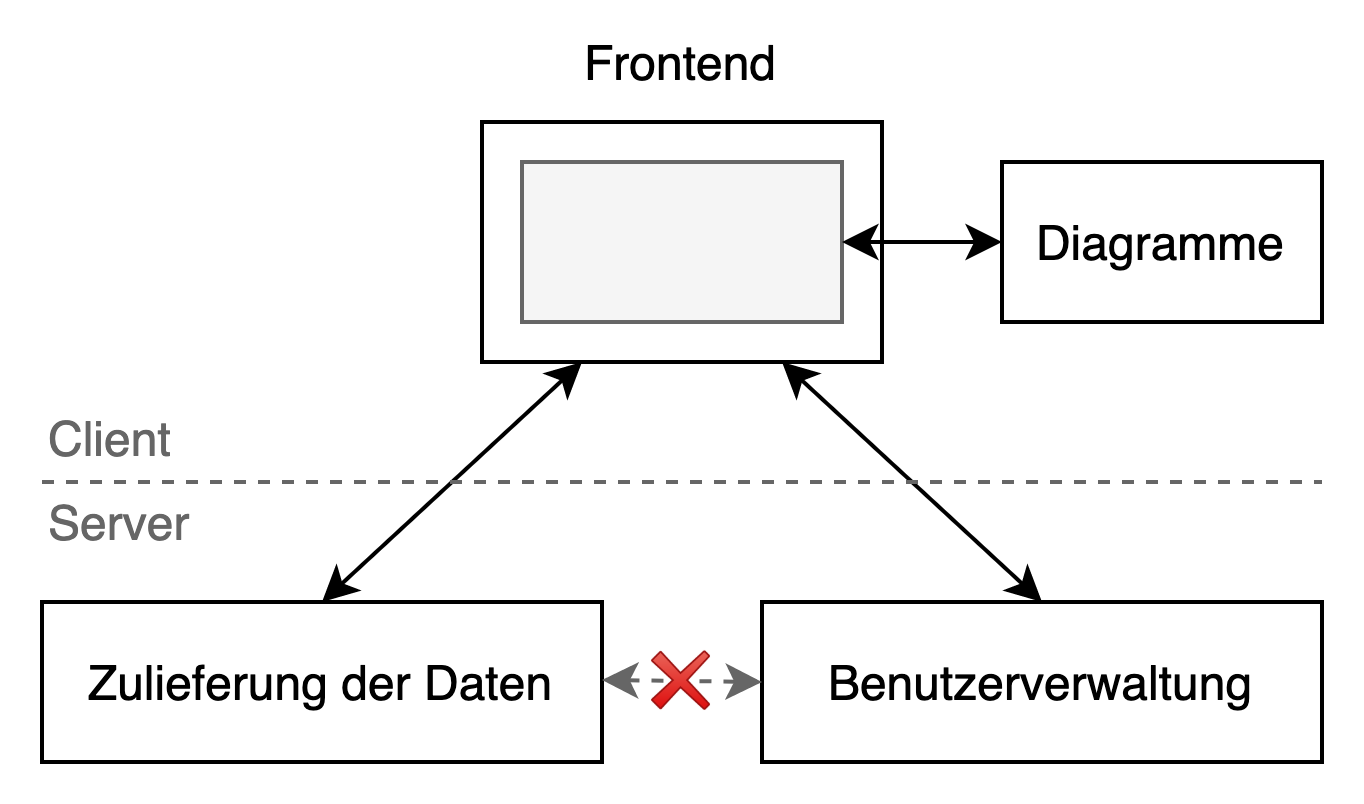
\includegraphics[scale=0.2]{img/abbildungen/TrennungDerLogic}
    \end{center}
    \caption{Trennung der Logic}
    \label{figure:trennungderlogic}
\end{figure}

Die Arbeit verfolgt auch für das Frontend einen Microservice-Ansatz. Man spricht hier von einem
Microfrontend. Michael Geers schreibt dazu in einem Artikel auf Digital Pioneers folgendes:
"Der Ansatz, der sich jetzt förmlich aufdrängt, ist die Umsetzung der Microservice-Idee
auch im Frontend. Anstatt einer ­großen Single-Page-Applikation baut man mehrere unabhängige
Teilapplikationen, die miteinander kommunizieren. Diese sind dann deutlich einfacher zu verstehen.
Der Einsatz einer neuen Technologie lässt sich in einem kleineren Rahmen testen."\cite{MicrofrontendT3N}
Dabei sollen die Diagramme eines Dashboards als einzelne Services ausgelagert werden (wie in Abbildung \ref{figure:trennungderlogic} dargetstellt).
Die Diagramme können so einzeln entwickelt und ausgeliefert werden. Aufgrund der
gleichen Machenschaft der Schnittstellen der Diagramme, kann man diese Art des Code-Splittings auch als
einen Plugin-Ansatz ansehen. Die Diagramme sollen über die In-Memory-Datenbank
Redis zur Verfügung gestellt werden. Die PWA selbst soll vorerst über einen
Nginx Webserver und später über ein CDN ausgeliefert werden. Die Diagramme werden mithilfe
von Dynamic Imports\footnote{Dynamic Imports gibt es seit ES6 (ECMAScript 2015)\cite{DynamicImportsV8}}
während der Laufzeit agil nachgeladen. Da immer nur die verwendeten Diagramme aus der In-Memory-Datenbank
geladen werden, kann die Webanwendung eine nahezu unendliche Auswahl an möglichen Diagrammen zur Visualisierung
der Daten bereitstellen.

\section{Diagrammanordnungsverfahren}
\label{sec:diagrammanordnungsverfahren}
Das Diagrammanordnungsverfahren beschreibt den Prozess, einzelne Diagramme in einem Dashboard anzuordnen.
Um das Verfahren zu vereinfachen, ist ein automatisches Anordnen der Diagramme diagonal sowie vertikal vorgesehen.
Die Anordnung der einzelnen Diagramme soll mithilfe der FlexBox Technologie implementiert werden.
\footnote{CSS Flexible Box Layout, bekannt als FlexBox, ist ein standardisiertes Anordnungsmuster, das von allen gängigen Browsern unterstützt wird.\cite{CanIUseFlexBox}}
Im mobilen Format sollen die einzelnen Diagramme untereinander aufgelistet werden. 

\begin{figure}
    \begin{center}
    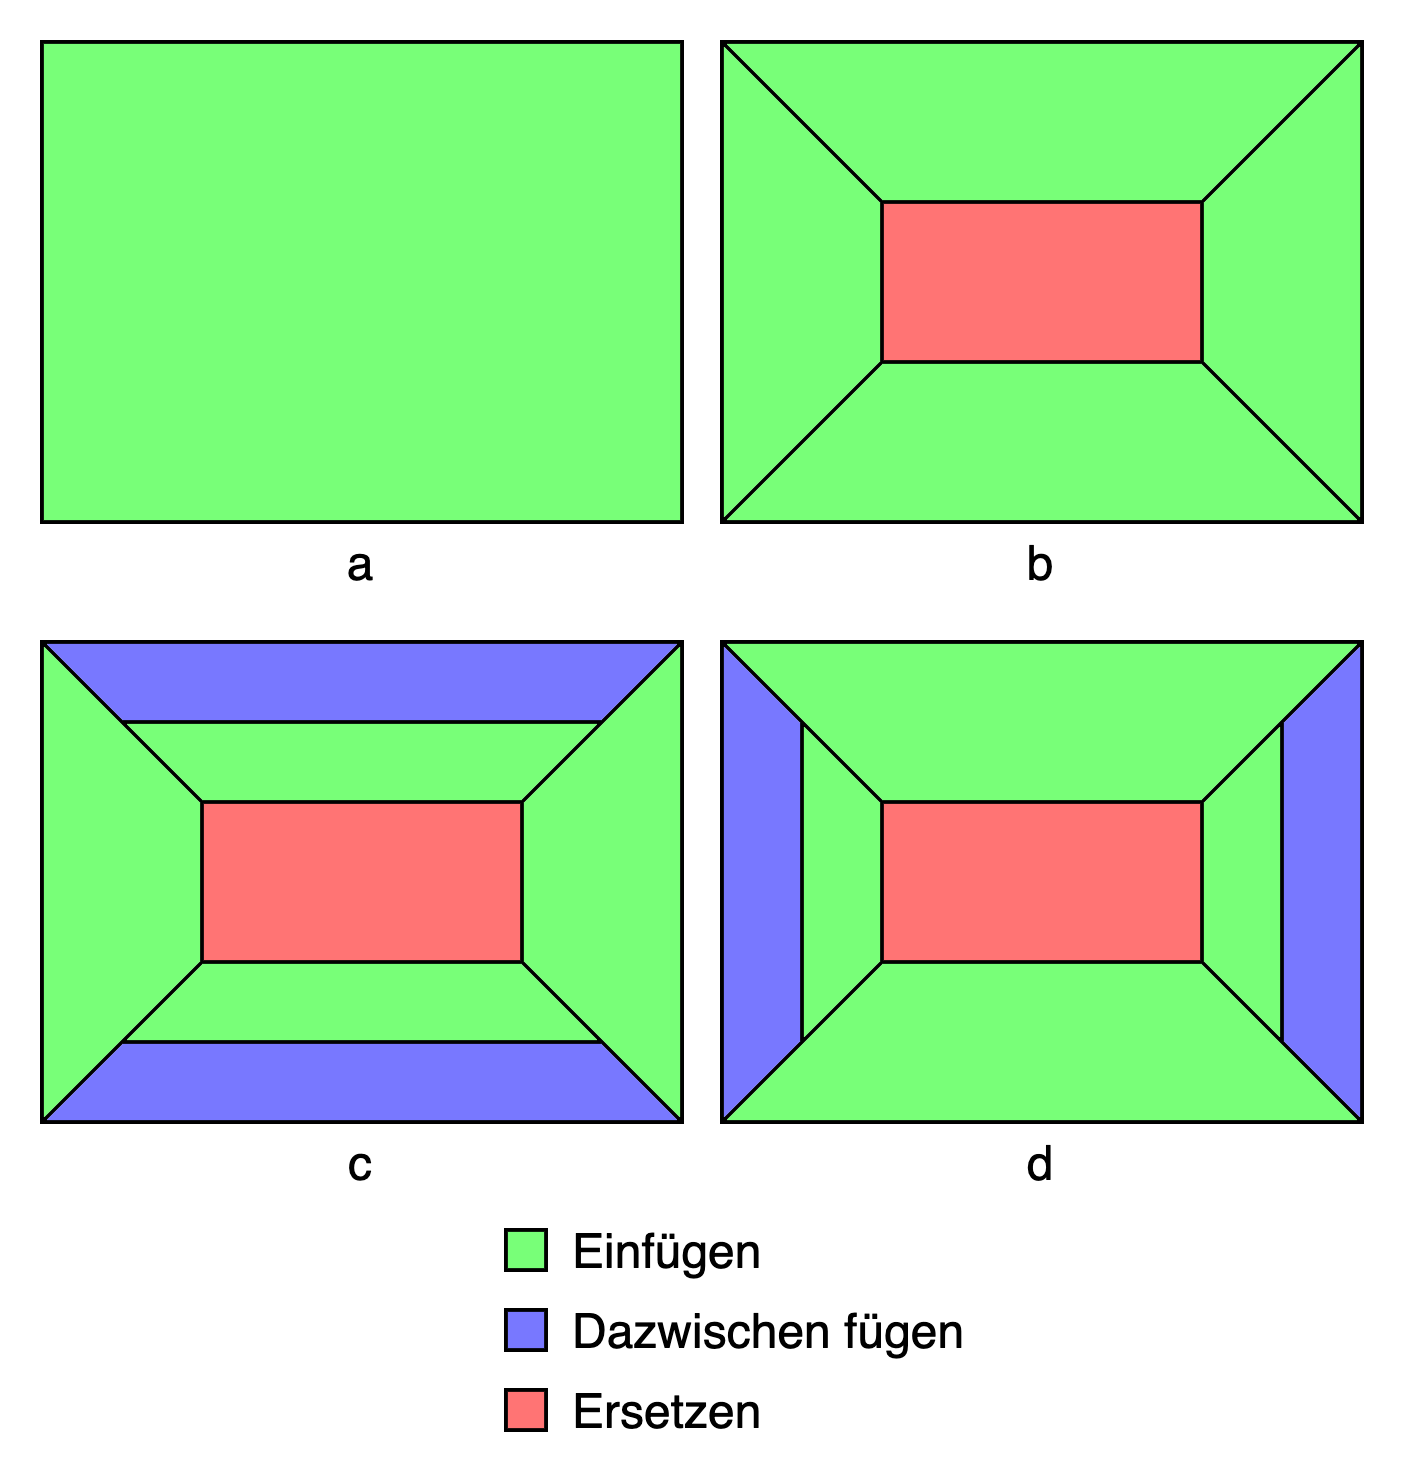
\includegraphics[scale=0.2]{img/abbildungen/DiagrammanordnungsverfahrenMitLegende}
    \end{center}
    \caption{Diagrammanordnunsverfahren}
    \label{figure:diagrammanordnungabbildung}
\end{figure}

Die Diagramme sollen nach und nach per Drag and Drop in das Dashboard integriert werden. Dieses Verfahren
wird in Abbildung \ref{figure:diagrammanordnungabbildung} dargestellt. \(a\) beschreibt den
initialen Zustand eines leeren Dashboards. Hier kann man durch Drag and Drop das erste Diagramm dem Dashboard
zuordnen. \(b\) beschreibt den Zustand des Dashboards mit genau einem enthaltenen Diagramm. Hier kann man das
neue Diagramm in alle Richtungen einfügen. Dabei Teilt das bestehende Diagram den Platz mit dem neuen gleichmäßig
auf. Bei der mittigen Positionierung wird das vorhandene Diagramm durch das neue ersetzt. \(c\) und \(d\)
beschreiben den Zustand, bei dem sich mehr als ein Diagramm im Dashboard befindet. Wenn man im Zustand \(b\)
ein Diagramm oberhalb oder unterhalb einfügt, bilden die beiden Diagramme eine Spalte. Beide dieser Diagramme
beinhalten nun den Zustand \(c\). Additional zu den möglichkeiten von Zustand \(b\), kann hier ein Diagramm
auch dazwischen gefügt werden. Es teilt sich dann den Platz mit den anderen Diagrammen in der Spalte.
Fügt man bei Zustand \(b\) ein Diagramm links oder rechts ein, bilden die beiden Diagramme eine Reihe.
Beide dieser Diagramme befinden sich nun in Zustand \(d\). Additional zu Zustand \(b\) können hier nun
auch neue Diagramme in der gleichen Reihe positioniert werden. Diese Reihen und Spalten können sich
immer weiter verschachteln. Somit kann der Benutzer mit einem ziemlich einfachen, intuitiven Verfahren
das Dashboard mit Diagrammen füllen. Durch einen Button in der Ecke rechts oben im Diagramm-Fenster
können diese auch wieder gelöscht werden. Dabei verhalten sich die zuvor beschriebenen Verfahren einfach rückläufig.
Die Anordnung der Diagramme wird als Baumstruktur im JSON-Format in der Datenbank persistiert.

\section{Strategie der vereinten Frontendanwendung}
\label{sec:vereintefrontendanwendung}
